\documentclass[12pt,a4paper]{report}
\usepackage[T1]{fontenc}
\usepackage{array}
\usepackage{mathptmx}
\usepackage[utf8]{inputenc}
\usepackage{amsmath}
\usepackage{amsfonts}
\usepackage{amssymb}
\usepackage{graphicx}
\usepackage{caption}
\usepackage{subcaption}
\usepackage{kpfonts}
\usepackage{hyperref}
\usepackage{graphicx}
\usepackage{natbib}
\usepackage{url}
\usepackage{float}
\usepackage{lscape}
\usepackage{algorithm}
\usepackage{algorithmic}
\usepackage[left=2cm,right=2cm,top=2cm,bottom=2cm]{geometry}
\def\thesection{\arabic{section}}
\def\thesubsection{\thesection.\arabic{subsection}}
\DeclareMathOperator*{\argmin}{\arg\!\min}
\setcounter{secnumdepth}{3}
\setlength{\parindent}{4em}
\setlength{\parskip}{1em}
\begin{document}
\begin{titlepage}
\begin{figure}
\hspace*{0.5cm}
\includegraphics[scale=0.9]{logos/logos1.pdf}
\end{figure}
   \vspace*{\stretch{0.2}}
   \begin{center}
   	\Huge\textbf{Annual Report}\\
   	\vspace*{2cm}
   	\Large\textbf{Control and Representation of Articulated Objects: Insights from robots}\\
   	\vspace*{2cm}
     \Large{PhD Program in Bioengineering Robotics}\\
     \Large{Curriculum: Cognitive Robotics, Interaction and Rehabilitation Technologies} \\ 
     \vspace*{2cm}
      \large{Student: Venkata Sai Yeshasvi Tirupachuri}\\
      \large{Cycle: XXXI}\\
      \vspace{0.1cm}
      \begin{frame}
      \small
      {\centering Tutors:\par}
      \begin{tabular}[t]{@{}l@{\hspace{3pt}}p{.6\textwidth}@{}}
             {\centering \hspace{0.9cm} Dr. Daniele Pucci} \\
             {\centering \hspace{0.1cm} Prof. Gabriel Baud-Bovy} \\
             {\centering \hspace{0.6cm} Prof. Guilio Sandini} \\
      \end{tabular}%
      \end{frame}
      
      \large{Year: 2}\\
      \large{EMail : \href{mailto:yeshasvi.tirupachuri@iit.it}{yeshasvi.tirupachuri@iit.it} \\ Mobile: +39-327-974-3351}
   \end{center}
   \vspace*{\stretch{2.0}}
\end{titlepage}
\tableofcontents
\pagebreak
\section{Research Activity}
\subsection{Scientific and Technological Objectives}

To be effective in an ever changing complex environments that humans live, robots need to have certain cognitive capabilities on par with humans. Most importantly fruitful interactions with the complex dynamic environment is very crucial. 

The research network PACE(Perception and Action in Complex Environments) deals with investigations into human motor control in highly complex environments. This is a fairly complex topic which can be explored at different fronts ranging from theoretical models to rehabilitation technologies. Coming from engineering and robotics background, I strongly believe that investigations in several areas of PACE research can result in endowing robots with humanlike cognitive capabilities for interaction with dynamic and complex environments. 

The prime case of complex environments considered in my research topic is articulated objects, like doors, scissors etc. Because of their structural rigidity, most robots strain to manipulate kinematically constrained articulated objects without causing large interaction forces. simply put these objects have different parts attached through joint(s) and hence the relative motion of the object parts is restricted according to the type of joint(s). We humans, with excellent perceptual and motor skills, learn to recognize and manipulate them easily. The same capability for robots is very much needed to be effective and productive in naturalistic environments. Hence the title of my topic is ``Control and Representation of Articulated Objects: Insights from robots". \\

The technical objectives can be summarized as 
\begin{itemize}
	\item A computational framework for articulation object model estimation
	\item Implementing cognitive models of sensorimotor signal processing in interaction 
	\item Validating the framework with experiments using humanoid iCub robot
\end{itemize}
\subsection{State of the art and Innovation}
State-of-the-art research in articulation model estimation has been mainly focused on exploting visual perception. For effective manipulation of articulation objects adequate information of the shape, pose and the kinematic structure of the objects and its parts is crucial. Pose tracking generally assumes the shape of the objects or object parts and utilizes segmentation in the visual input. Shape reconstruction can be achieved using integration of multiple poses and then the kinematic structure of an articulated object can be achieved using the above information on the object parts.

The segmentation problem deals with extracting the region of interest in the visual input which contains the object to track. 
\begin{itemize}
	\item Single image based segmentation ~\cite{mishra2009active},~\cite{papon2013voxel}
	\item Motion based segmentation ~\cite{chien2002efficient}
\end{itemize}

Pose estimation or visual tracking can be achieved using
\begin{itemize}
	\item Based on a known shape model of the object ~\cite{wuthrich2013probabilistic}
	\item Based on the sufficient texture extracting features ~\cite{martin2014online} or optical flow ~\cite{stuckler2013efficient},~\cite{ochs2014segmentation}
\end{itemize} 

Shape reconstruction outputs a 3D model of an object by stitching together several object views into one coherent shape model using relative poses w.r.t the visual system. Object views are obtained using information from segmentation and pose estimation~\cite{krainin2011manipulator}. Visual SLAM is a popular approach combining tracking and shape reconstruction but for an entire scene that is assumed to be static. An integrated approach for the visual perception of articulated objects is recently proposed in ~\cite{martinintegrated} which combines tracking, shape reconstruction and estimation of kinematic structures. 

Doors are the most likely experienced articulated objects in many robotic applications like rescue scenarios, elderly care, hospitality etc., and the earliest investigations started with a simple strategy to open an unknown door ~\cite{niemeyer1997simple}. More recently, Advait Jain and Charles C. Kemp proposed the concept of equilibrium point control (EPC) ~\cite{jain2009pulling} for the specific task of opening novel doors and drawers. In addition they implemented an articulation model estimation algorithm using the end-effector trajectory, assuming a stable grasp and planar motion of the end-effector. The algorithm returns an estimate of the location of the axis of rotation and the radius. Prismatic joint is estimated as a rotational joint with large radius. 

Dov Katz and Oliver Brock ~\cite{katz2007interactive} introduced the idea of interactive perception paradigm and highlights the need for extracting task specific perceptual information using the manipulation capabilities of a robot by interacting with the environment. Some of the limitations in \cite{katz2007interactive} are removed in ~\cite{katz2008manipulating} and a robust algorithm is presented. Feature trajectories of moving objects are extracted using optical flow based tracking and a graph is built where vertices represent the tracked features. Highly connected sub-graphs are separated using min-cut algorithm and these sub-graphs represent the object parts. Then the articulation models are extracted from the information contained in the graph. Rotational joint is identified by rotating centers between two sub-graphs and prismatic joint by shifting movements of sub-graphs. They successfully demonstrated the use of interactive perception in extracting kinematic model of various tools to build a Denavit-Hartenberg (DH) parameter model and then use it to operate a tool. Furthermore, a symbolic learning based approach to manipulate is presented in ~\cite{brock2009learning} which uses relational representations of kinematic structures that are grounded using perceptual and interaction capabilities of the robot. They successfully demonstrated learning and generalization of manipulation knowledge to previously unseen objects. 

Strum et al. ~\cite{sturm2009learning} proposed a probabilistic learning framework using noisy 3D pose observations of object parts. They implemented predefined candidate joint models with parameters and also a non-parametric gaussian process model to which observed 3D pose trajectory data of object parts is fit to find kinematic structures of kinematic trees. Unlike the previous works this is a passive approach and they use pose observations from motion capture system, when the articulated object is manipulated by someone, and simulated data to validate their framework. Further, a stereo camera system is used to get dense depth images as input ~\cite{sturm20103d}. An approach to direct interaction with articulated objects to learn articulation models and improve based on experience is presented in ~\cite{sturm2010operating}. Furthermore, a unified framework with several extensions like dealing with kinematic loops and extended set of experiments is presented in ~\cite{sturm2011probabilistic}.

Stefan et al. ~\cite{otte2014entropy} introduced the exploration challenge for robots where the task is to perform explorative actions and learn the structure of the environment. One of their main contributions is probabilistic belief representation of articulation models including properties like friction and joint limits. They successfully demonstrated how the behaviour emerged from entropy-based exploration is more informative than explorative strategies based on heuristics. Hausman et at. ~\cite{hausman2015active} proposed a partcile filter based approach where the articulation models are represented as particles and implemented a probabilistic framework based on the concept of interactive perception to integrate visual observations with manipulation feedback from the robot. They also presented best action selection methods based on entropy and information gain which guides the robot to perform the most useful interactions with the object to reduce its uncertainty.

Martin-Martin Roberto and Oliver Brock ~\cite{martin2014online} presented an online multi-level recursive estimation algorithm considering task-specific priors based on the concept of interactive perception. They used series of RGB-D image data as input to estimate articulation models including the joint configuration. Furthermore, they extended their approach ~\cite{martin2017building} integrating information from vision, force-torque sensing and proprioception. In addition to kinematic model estimation they also generated a dynamic model of the articulated object. 

The choice of a well established framework on human motor control to facilitate the basic software infrastructure for my research is a crucial step. Towards this end I did review of papers on the framework of Active Inference ~\cite{friston2015active},~\cite{friston2011action} put forward by Prof. Karl Friston. Also I studied the framework of Passive Motion Paradigm(PMP) ~\cite{mohan2011passive}, ~\cite{mohan2013inference} championed by our colleagues Dr. Vishwanathan Mohan and Prof. Pietro Morasso from the Italian Institute of Technology.

Visual information has been used as the most dominant sensory modality in articulation model estimation. But while manipulating an articulated object, another key information available is the interaction wrench. As a part of the Dynamic Touch and Interaction team and in collaboration with Dynamic Interaction Control  team, I am  exploring the possibilities of using interaction wrench along with visual perception  to estimate the kinematic structure and dynamic properties of articulated objects. From the visual perception kinematic properties of the artiulated can be estimated but by also using interaction wrench information we believe one can estimate the dynamic properties too. This facilititates for better control during object manipulation. A bayesian framework is proposed in ~\cite{nori2015simultaneous} for simultaneous state and dynamics estimation in presence of multiple redundant sensory information. But in the case of manipulation of articulated objects state information will estimated using visual inputs. 
 
\subsection{Methodology and Workplan}
\subsubsection{Modelling}

We modelled two simple artitulated objects using Simulation Description Format (SDF) to be used in Gazebo simulation environment. The objects contain two links connected through a \textit{prismatic} joint, \textit{\textbf{P}} in one (Fig. \ref{pmodel}) and a \textit{revolute} joint, \textit{\textbf{R}} in the other  (Fig. \ref{rmodel}). The reasoning behind this modelling is that most real life articulated objects can be represented in this simplified form. The cylindrical elements in black color are the handle links and the rectangular elements in yellow color are articulated object links. The handle links of the articulated objects are connected to object links through a fixed joint and one of the handles is anchored to the world in gazebo through a fixed joint and this also anchors the object link attached to that handle. The reasoning behind this choice is that many articulated objects have one of their links either grounded or are quite heavy to move compared to the freely movable link. 

\begin{figure}[H]
	\begin{subfigure}[b]{0.5\textwidth}
		\centering
		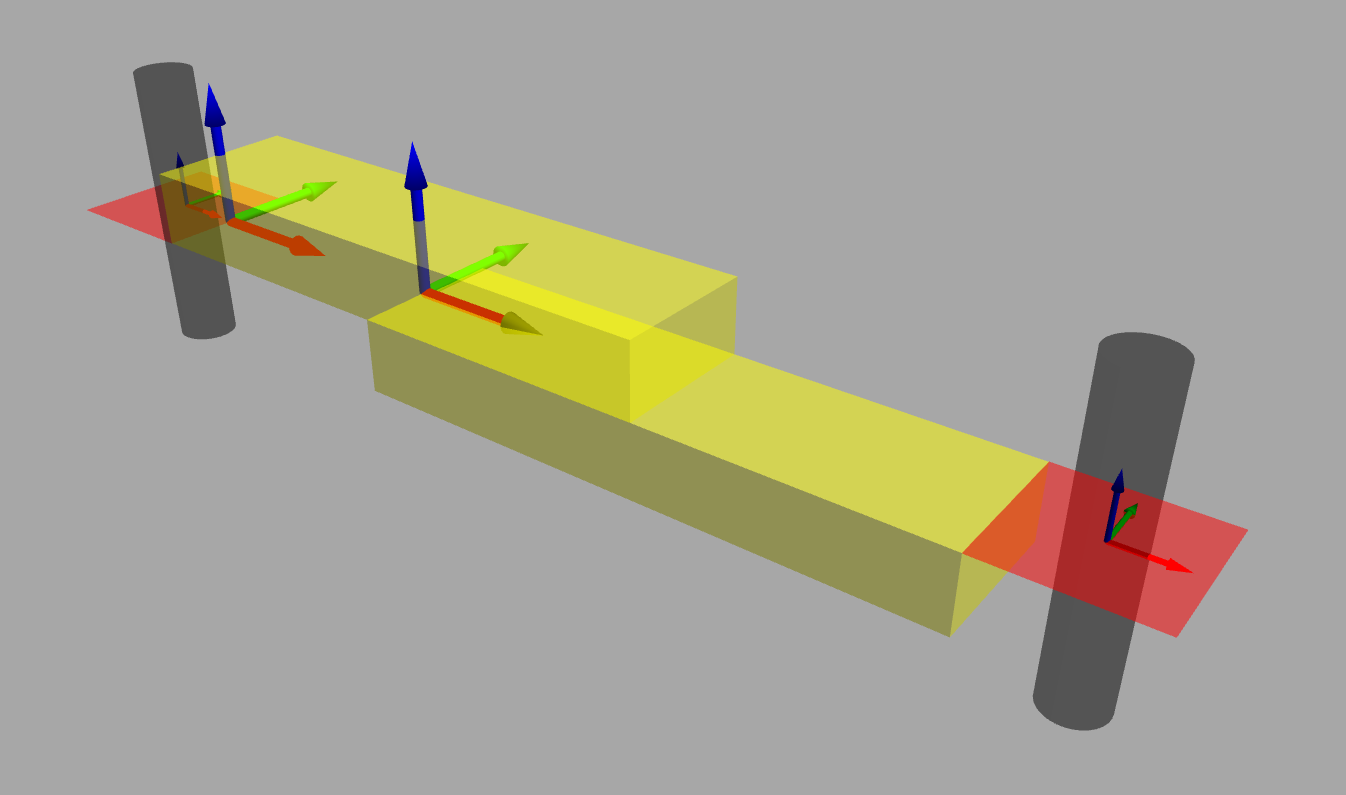
\includegraphics[scale=0.15]{figures/1p_2link.png}
		\caption{Prismatic Model}
		\label{pmodel}
	\end{subfigure}
	\begin{subfigure}[b]{0.5\textwidth}
		\centering
		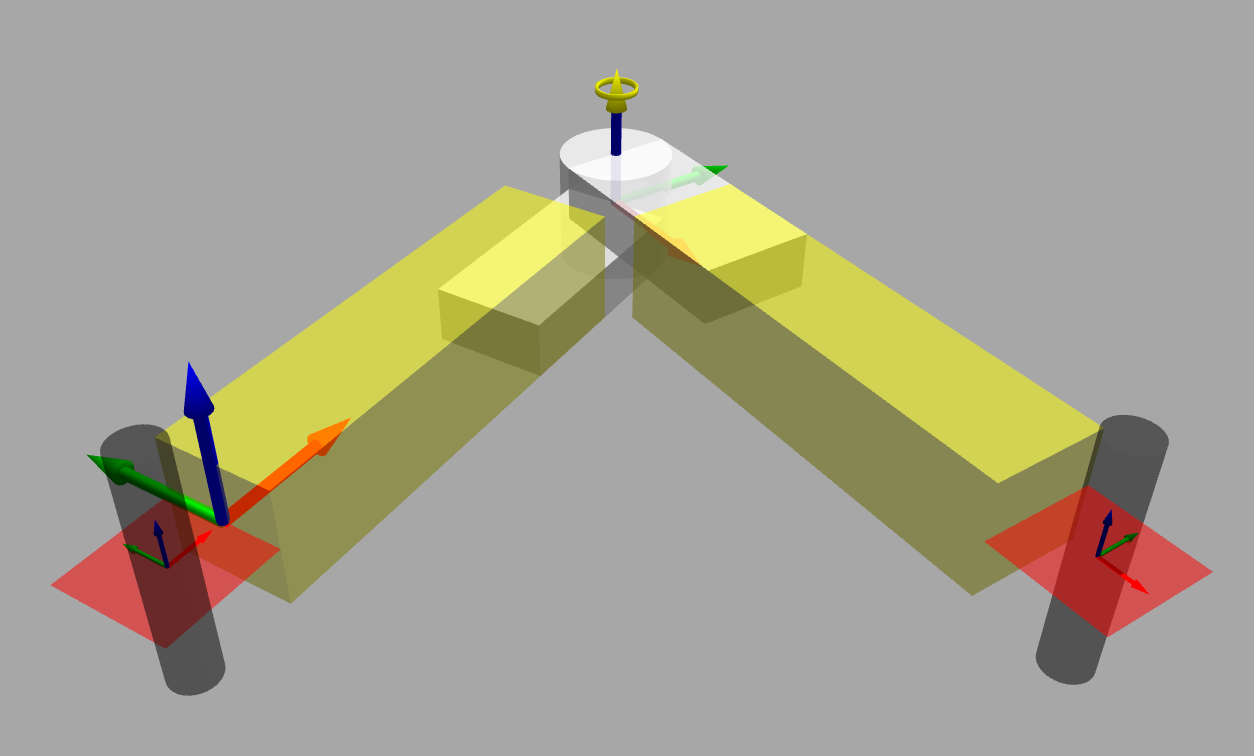
\includegraphics[scale=0.16]{figures/1r_2link.png}
		\caption{Revolute Model}
		\label{rmodel}
	\end{subfigure}
	\caption{Articulated Object Models}
	\label{objects}
\end{figure}

\subsubsection{Experimental Scenario}
The experimental scenario we want to test is as indicated in the figure \ref{icub_object}, where the icub robot is holding the articulated object at the handles and performs explorative actions to estimate the
articulation model present between the links.

\begin{figure}[H]
	\begin{subfigure}[b]{0.5\textwidth}
		\centering
		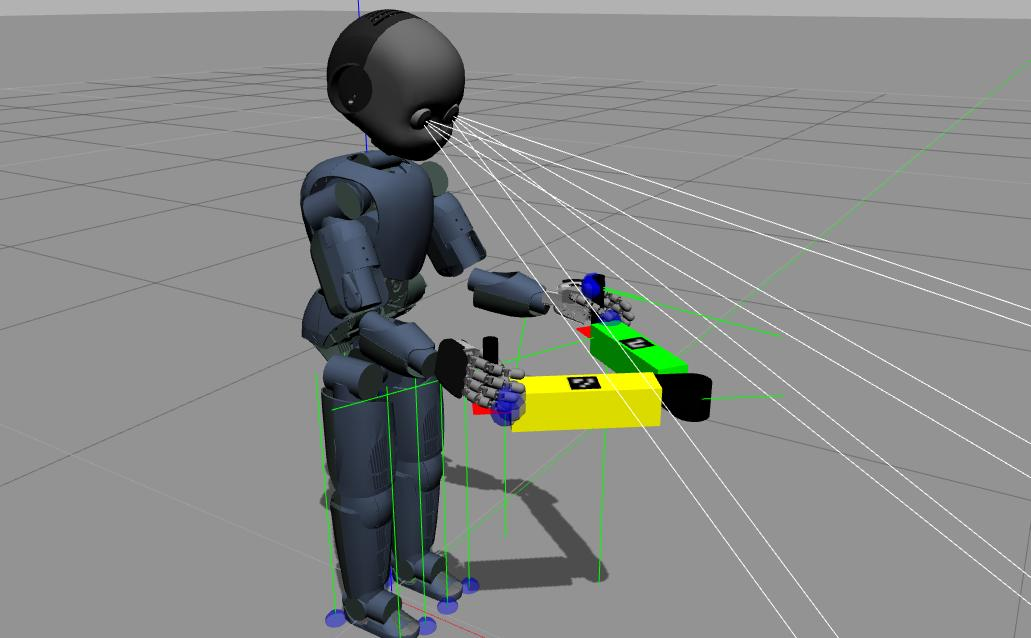
\includegraphics[scale=0.22]{figures/icub_object_side.jpg}
		\caption{Side View}
		\label{icub_object_side_view}
	\end{subfigure}
	\begin{subfigure}[b]{0.5\textwidth}
		\centering
		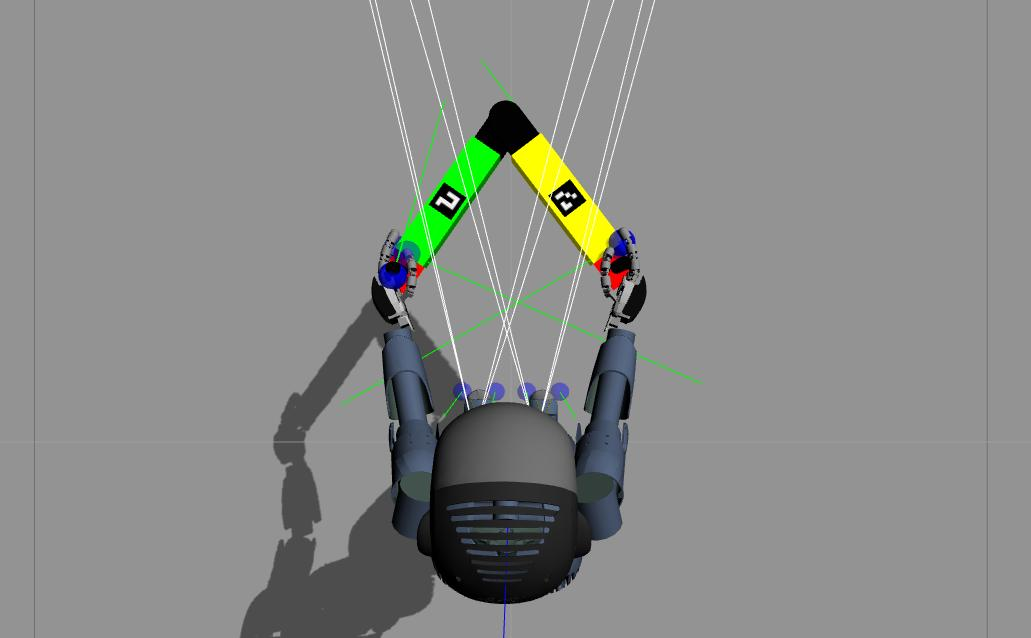
\includegraphics[scale=0.22]{figures/icub_object_top.jpg}
		\caption{Top View}
		\label{icub_object_top_view}
	\end{subfigure}
	\caption{Experimental Scenario: iCub manipulating an articulated object}
	\label{icub_object}
\end{figure}

\subsubsection{Implemetation Details}
\subsubsection*{Visual Perception}
I started working on the submodules of vision and force-torque in the perception module of the software architecture shown in figure \ref{SoftArc}. Obtaining robust 3D pose values of rigid bodies is still an open challenge in the field of computer vision. Vast amount of research has been carried on tracking rigid bodies either using markers, features or depth information. As visual perception is not the main goal of this work, I made use of aruco library ~\cite{Aruco2014} which is an opensource software for augumented reality applications based on OpenCV. Figure \ref{markersboard} shows an array of markers and figure \ref{marker_stapler} shows the markers attached on the two moving parts of a stapler with their detected 3D pose shown with axes.

\begin{figure}[H]
	\centering
	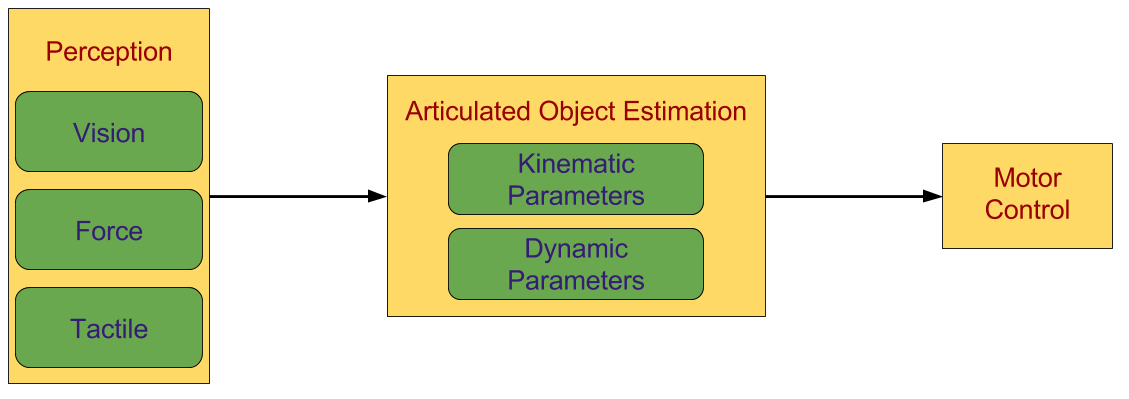
\includegraphics[scale=0.3]{figures/SoftwareArch_year1.png}
	\caption{Software Architechture}		
	\label{SoftArc}
\end{figure}

\begin{figure}[H]
	\begin{subfigure}[b]{0.5\textwidth}
		\centering
		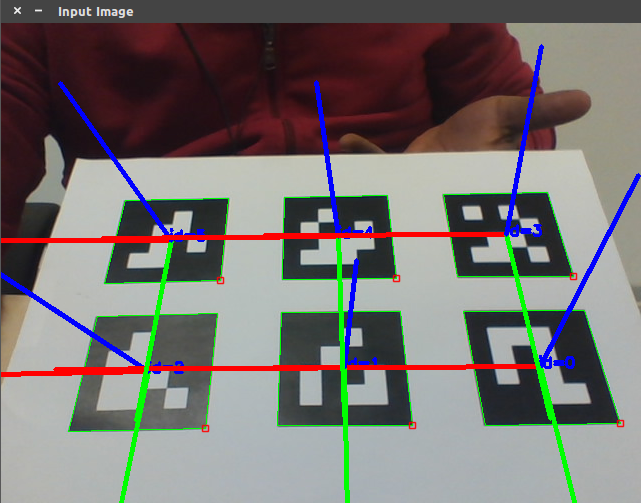
\includegraphics[scale=0.3]{figures/markersboard.png}
		\caption{Markers Board}
		\label{markersboard}
	\end{subfigure}
	\begin{subfigure}[b]{0.5\textwidth}
		\centering
		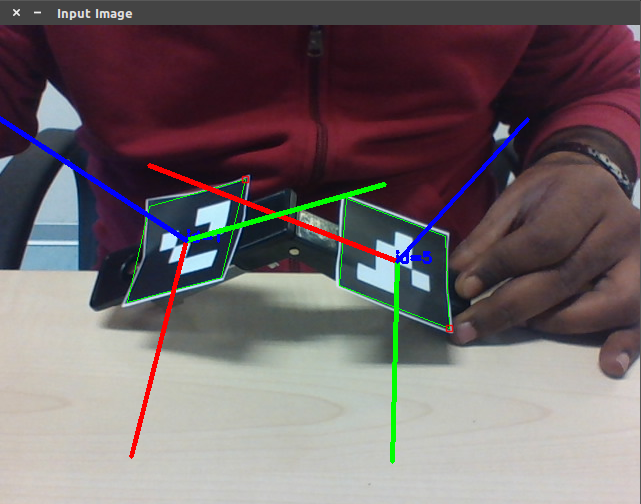
\includegraphics[scale=0.3]{figures/stapler.png}
		\caption{Markers on a stapler}
		\label{marker_stapler}
	\end{subfigure}
	\caption{Augumented Reality Markers}
	\label{armarkers}
\end{figure}

\subsubsection*{Wrench Perception}
Coming to force-torque perception, iCub robot is equipped with six proximal six-axis F/T sensors as shown in the figure \ref{icub_ft}. While using the iCub robot external wrenches can be estimated using the techniques develoed for whole-body control ~\cite{nori2015icub}. At this point the current icub model described using an URDF (Universal Robot Description Format) file in simulation environment did not include the hands of the robot. I created new URDF files ~\cite{icub_hands_urdf} for the hands of the robot along with collision elements and accomplished contact tuning ~\cite{icub_hands_contact_tuning} in gazebo simulation environment. Later two frames as shown in the figure \ref{hands_frames} are defined at the center of the hands at which we can estimate the wrench acting on the robot. 

\begin{figure}[H]
  \centering
  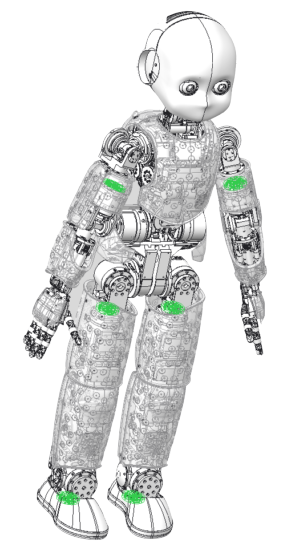
\includegraphics[scale=0.5]{figures/icub_ft.png}
  \caption{iCub robot: location of six proximal F/T Sensors}
  \label{icub_ft}
\end{figure}

\begin{figure}[H]
	\begin{subfigure}[b]{0.5\textwidth}
		\centering
		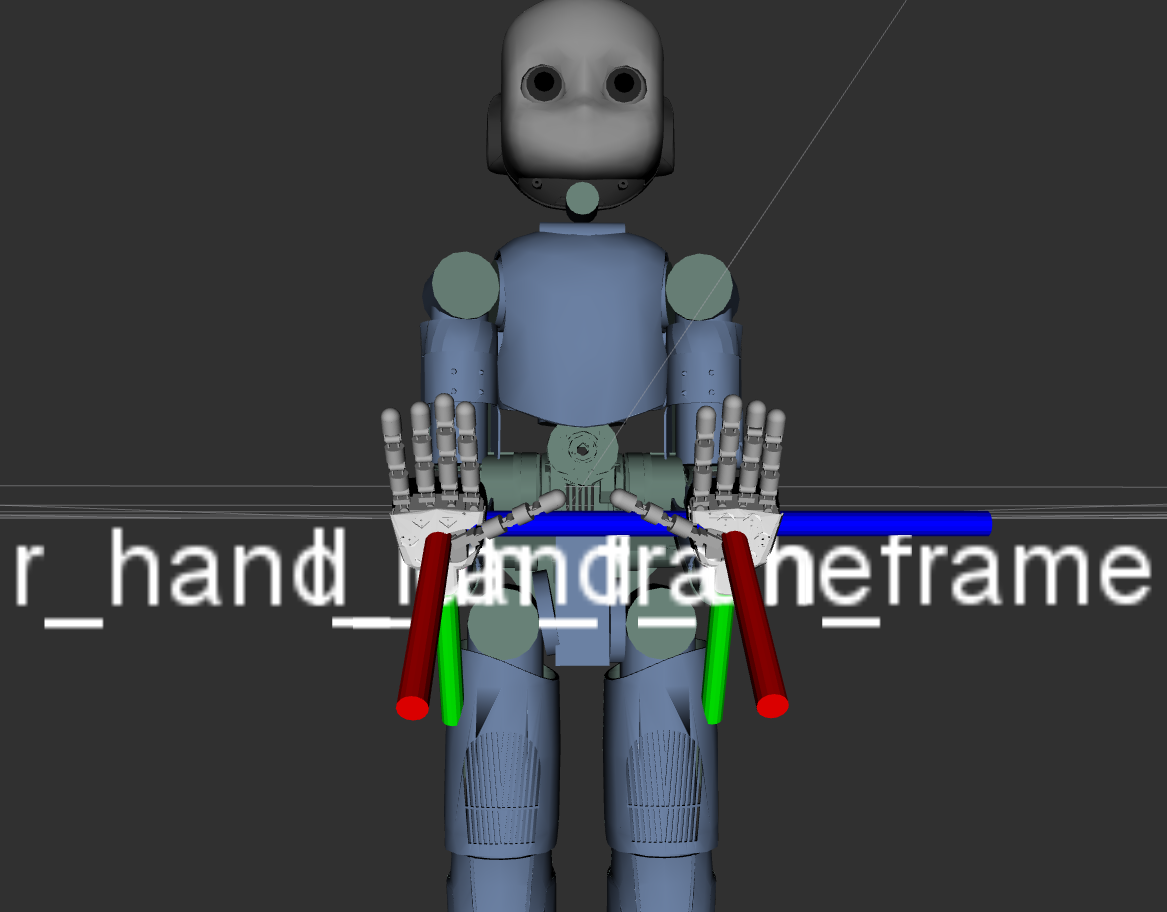
\includegraphics[scale=0.21]{figures/hands_front.png}
		\caption{Front View}
		\label{hands_front_view}
	\end{subfigure}
	\begin{subfigure}[b]{0.5\textwidth}
		\centering
		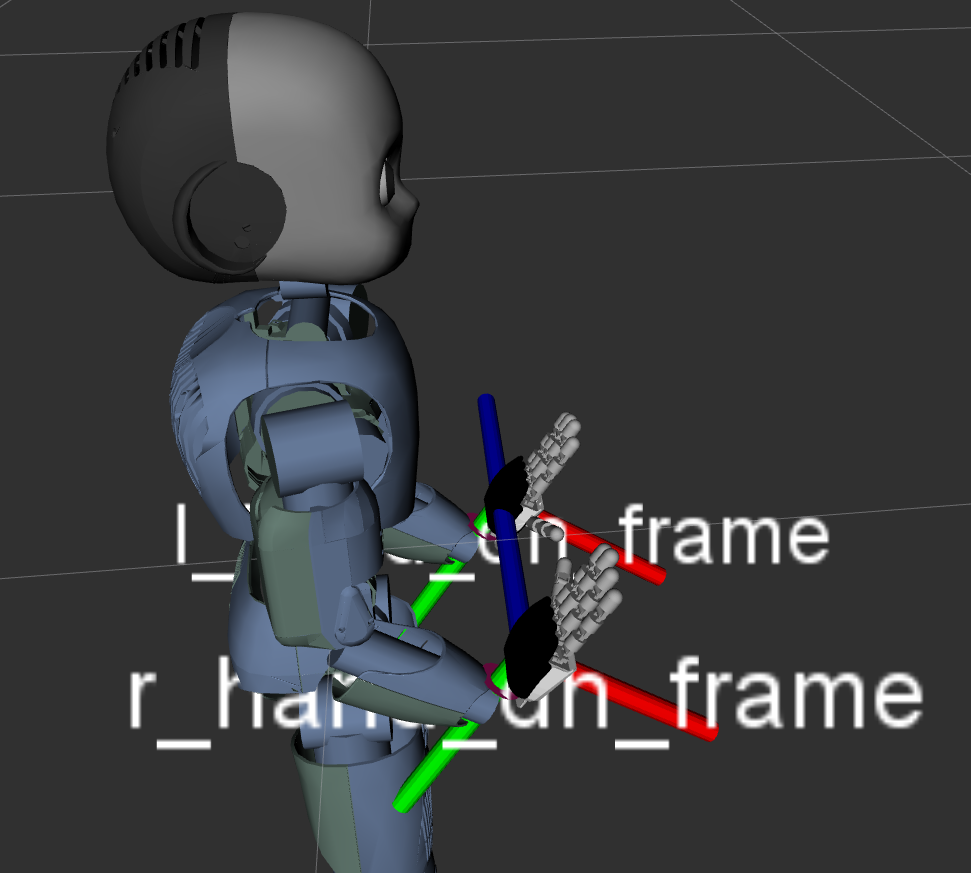
\includegraphics[scale=0.22]{figures/hands_side.png}
		\caption{Side View}
		\label{hands_side_view}
	\end{subfigure}
	\caption{iCub hands with new frames}
	\label{hands_frames}
\end{figure}

A simulated 6 axis Force-Torque sensor plugin ~\cite{hoffman2014yarp} is placed at the fixed joint connecting object link to its handle, to measure the external wrenches acting on the object links. In an ideal case where the iCub robot is having a stable power grasp of the object, the wrench measurements read from this Force-Torque sensor plugin should be similar to the measurements obtained at the hands of the robot, provided that the direction of measurement is the same. But in practice the hands of the iCub robot are quite complex to achieve a stable power grasp.

\subsubsection*{Articulation Estimation Algorithm}

Visual information has been used as the most dominant sensory modality in articulation model estimation. But while manipulating an articulated object, another key information available is the interaction wrench. We came up with an articulation estimation algorithm that uses momentum information and the interaction wrench information.

In this work we use spatial vectors ~\cite{featherstone2014rigid}, which are 6D vectors that are proven to be a powerful tool to analyse rigid-body dynamics. Unlike the standard notation of spatial vectors, in the spatial motion vectors we use the linear part first followed by the angular part and in the spatial force vectors we use the forces first followed by the moments. In a complex articulated system consisting of several links connected through joints of several degrees of freedom (e.g humanoid robots), the total momentum of the system is the sum of link momenta, provided that the link momenta are expressed in a common reference frame. For humanoid robots, it is commonly expressed after projecting each link momenta to the robot's Center of Mass (CoM, $G$) and hence it is called centroidal momentum ~\cite{orin2013centroidal}. 
\begin{equation}
  ^Gh=\sum\limits_{i=1}^n \ ^GX_i \ h_i = \sum\limits_{i=1}^n \ ^GX_i \ M_i \ \mathrm{v}_i
\end{equation}
Where, 
\begin{itemize}
  \item $^Gh$ is the centroidal momentum of the system.
  \item  $n$ is the total number of links in the articulated system.
  \item $^GX_i$ is the spatial transformation from the body reference frame to the center of mass of the system. 
\end{itemize}

For our modelling, the total momentum of the articulated object expressed with respect to the inertial frame of reference is given by,
\begin{equation}
  h =  X_1 \ M_1 \ \mathrm{v}_1 + X_2 \ M_2 \ \mathrm{v}_2
 \label{totalMom}
\end{equation}

In the case of a rigid body system containing a kinematic tree structure, the velocity of a body $i$, expressed in its body frame, is given by,
\begin{equation}
  \mathrm{v}_i = \  ^iX_{\lambda(i)} \ \mathrm{v}_{\lambda(i)} + \mathrm{v}_{Ji}
  \label{generalBodyVel}
\end{equation}
where,
  \begin{itemize}
    \item $\mathrm{v}_i$ is the twist of the $i$-th link expressed in its body frame.
    \item $\mathrm{v}_{\lambda(i)}$ is the twist of the parent link of $i$-th link, expressed in its body frame. 
    \item $^iX_{\lambda(i)}$ is the spatial transformation from the parent link to the child link.
    \item $\mathrm{v}_{Ji}$ is the twist of the $i$-th joint, connecting link $i$ to its parents, expressed in the body frame of link $i$.
  \end{itemize}
   
  The equation(\ref{generalBodyVel}), in our modelling, simplifies to,
  \begin{equation}
    \mathrm{v}_2 = \  ^2X_{1} \ \mathrm{v}_{1} + \mathrm{v}_{J}
  \label{bodyVel}
  \end{equation} 
  
   The twist of a joint, expressed in the child link body frame, is given by,
  \begin{equation}
    \mathrm{v}_{J} = \mathrm{S}\dot{q}
    \label{jointVel}
  \end{equation}
  
  In this work we considered only prismatic and revolute articulation models as they are present in most articulated objects. Assumming these two articulation model types we compute two joint twist quantities, using the relative transformation between the fixed link and movable link. In case of prismatic model hypothesis, the joint velocity $\dot{q}_p$ and the joint axis $\mathrm{S}_P$ are computed from the linear part of the relative transformation. In case of a revolute model hypothesis, the joint velocity $\dot{q}_R$ and the joint axis $\mathrm{S}_R$ are computed from the rotation matrix of the relative transformation. 
  
  Now while computing the total momentum using equation(\ref{totalMom}), the information of articulation \textit{model} is encapsulated, which can be represented in short as
  \begin{equation}
    h(model)
  \end{equation}
  
  The total wrench acting on a system, expressed in the inertial frame $A$, is given by the summation of external wrenches and gravitational forces on each link.  
\begin{equation}
  W=\sum\limits_{i=1}^l \ ^AX_i \ \text{f}_i + \sum\limits_{j=1}^n \ ^AX_j \ m_jg
\label{generalTotalWrench}
\end{equation}
where,
\begin{itemize}
  \item $l$ is the number of force-torque sensors present in the articulated object.
  \item $\mathrm{f}_i$ is the total wrench measured by a force-torque sensor expressed in its local frame of reference.
  \item $^AX_i$ is the spatial transformation from the force-torque sensor local frame to the inertial frame, $A$.
  \item $^AX_j$ is the spatial transformation from the body referece frame $B$ to the inertial frame, $A$.
\end{itemize}

In our modelling, the equation(\ref{generalTotalWrench}) is reduced to,
\begin{equation}
  W= X_{ft_1}\text{f}_1 + X_{ft_2}\text{f}_2 +  X_{com_1}m_1g + X_{com_2}m_2g
\label{TotalWrench}
\end{equation}

 For any rigid body system, the sum of the external wrenches acting on it is equal to the rate of change of momentum. 
\begin{equation}
  W=\dot{h}(model)
  \label{relation}
\end{equation}

  Considering the two articulated model hypotheses, the model which solve the following optimization represents the true joint nature of articulation present between the two object parts.
  \begin{equation}
    model^*= \argmin\limits_{model}\sum||W-\dot{h}(model)||
  \end{equation}
  
Currently our algorithm \ref{alg:joint estimation} is offline and the recorded data is passed as input. All the quantities denoted in the algorithm are computed with respect to the inertial frame of reference, A. The algorithm outputs two quantities,
\begin{itemize}
  \item \textit{Prismatic Hypothesis Error}, which is the value that corresponds to the mismatch between the actual prismatic joint motion and the prismatic articulation model hypothesis,
  \begin{equation}
    P_{hyp}= \sum\limits_{data}||W-\dot{h}(prismatic ~model)||
    \label{phyp}
  \end{equation}
  
  \item \textit{Revolute Hypothesis Error} $(Rhyp)$ which is the value that corresponds to the mismatch between the actual revolute joint motion and the revolute model hypothesis,
  \begin{equation}
    R_{hyp}= \sum\limits_{data}||W-\dot{h}(revolute ~model)||
    \label{rhyp}
  \end{equation}
\end{itemize}

\begin{algorithm}[H]
    \caption{Calculate Joint Hypothesis - $P_{hyp}$, $R_{hyp}$}
    \label{alg:joint estimation}
    \begin{algorithmic}[1]
        \REQUIRE: $Data : t, \textit{P}_1, \textit{P}_2, \mathrm{f}_1,\mathrm{f}_2$ 
  
        \FOR{$i < size(Data,1)$}
        
           %%Time                            
           \STATE $dt$ $\leftarrow$ $diff(t)$
           
           %\FOR{$i < size(batch,1)$}
             
             %%Relative Transformation
             \STATE $T_1$ $\leftarrow$ $H(P_1)$
             \STATE $T_2$ $\leftarrow$ $H(P_2)$
             \STATE $^1T_2$ $\leftarrow$ $T_1^{-1}$ $T_2$
            
             %%Prismatic Joint Quantities
             \STATE $^1P_2$ $\leftarrow$ $linear(^1T_2)$
             \STATE $q_P$ $\leftarrow$ $norm(^1P_2)$
             \STATE $\mathrm{S}_P$ $\leftarrow$ $\begin{bmatrix}
                                                   \frac{^1P_2}{d},0,0,0
                                                \end{bmatrix}^T$
                                                
             \STATE $\dot{q}_P$ $\leftarrow$ $\frac{diff(q_P)}{dt}$ \hspace*{4.5cm} 
             \STATE $\mathrm{v}_J^P$ $\leftarrow$ $X(T_1)$ $\mathrm{S}_P \ \dot{q}_P$ \hspace*{3.4cm}\hspace{-3.2cm}
             
             %%Revolute Joint Quantities                                    
             \STATE $^1{R}_2$ $\leftarrow$ $rot(^1T_2)$
             \STATE $axisAngleVector$ $\leftarrow$ $vrrotmat2vec(^1R_2)$
             \STATE $q_R$ $\leftarrow$ $axisAngleVector(4)$
             \STATE $\mathrm{S}_R$ $\leftarrow$ $\begin{bmatrix}
                                                  0,0,0,axisAngleVector(1:3)
                                                \end{bmatrix}^T$
             \STATE $\dot{q}_R$ $\leftarrow$ $\frac{diff(q_R)}{dt}$   
             \STATE $\mathrm{v}_J^R$ $\leftarrow$ $X(T_1)$ $\mathrm{S}_R \ \dot{q}_R$
             
             %%Body 1 Velocity
             %%Linear Velocity
             \STATE $p_1$ $\leftarrow$ $linear(T_1)$
             \STATE $v_{1}$ $\leftarrow$ $\frac{diff(p_1)}{dt}$
        
             %%Angular Velocity
             \STATE $R_1$ $\leftarrow$ $rot(T_1)$
             \STATE $\dot{R}_1$ $\leftarrow$ $\frac{diff(R_1)}{dt}$
             \STATE $\omega_{1}$ $\leftarrow$ $\dot{R}_1 \ R_1^T$
             
             %%Spatial Velocity
             \STATE $\mathrm{v}_1$ $\leftarrow$ $[v_{1},\omega_{1}]^T$
               
             %%Body 2 Velocity
             \STATE $\mathrm{v}^P_2$ $\leftarrow$ $\mathrm{v}_1$ $+$ $\mathrm{v}_J^P$
             \STATE $\mathrm{v}^R_2$ $\leftarrow$ $\mathrm{v}_1$ $+$ $\mathrm{v}_J^R$
        
        
             %%System Momentum
             \STATE $h^P$ $\leftarrow$ $[{X}_1^* \ M_1 \ ^1{X}] \ \mathrm{v}_1$ $+$ $[{X}_2^* \ M_2 \ ^2{X}] \ \mathrm{v}_2^P$
             \STATE $h^R$ $\leftarrow$ $[{X}_1^* \ M_1 \ ^1{X}] \ \mathrm{v}_1$ $+$ $[{X}_2^* \ M_2 \ ^2X] \ \mathrm{v}_2^R$
             
             %%Rate of change of momentum
             \STATE $\dot{h}^P$ $\leftarrow$ $\frac{diff(h^P)}{dt}$
             \STATE $\dot{h}^R$ $\leftarrow$ $\frac{diff(h^R)}{dt}$
             
             %%Spatial Wrench        
             \STATE $\text{f}_1$ $\leftarrow$ $X_{left}^*$ $\text{f}_1$
             \STATE $\text{f}_2$ $\leftarrow$ $X_{right}^*$ $\text{f}_2$
             \STATE $W$ $\leftarrow$ $\text{f}_1 + \text{f}_2 + {X_{{com}_1}^*} m_1 \text{g} + {X_{{com}_2}^*} m_2 \text{g} $
             
             \newpage
             
             %%Hypothesis
             \STATE $P$ $\leftarrow$ $W$ $-$ $\dot{h}^P$
             \STATE $R$ $\leftarrow$ $W$ $-$ $\dot{h}^R$
        
           
           %\ENDFOR
           
        \ENDFOR    
        \STATE $P_{hyp}$ $\leftarrow$ $norm(sum(P.^*P))$ 
        \STATE $R_{hyp}$ $\leftarrow$ $norm(sum(R.^*R))$      
    \end{algorithmic}
\end{algorithm}




\subsection{Achieved results, dissemination, deviation from the original plan}
The gantt chart in the figure \ref{gantt} shows the proposed work plan during the project proposal and the actual work progress during the first year of PhD. The software architecture indicated in the figure \ref{SoftArc} is realized by implementing various submodules to a functional level that enabled us to perform our experiments in gazebo simulation environment.

We encountered a couple of problems to conduct intented experiments. Firstly, the 3D pose values of the object links using markers is inconsistent, particularly the orientation part. This is due to the noisy visual observations. Secondly, as mentioned before the hands of the iCub robot are quite complex to maintain a stable power grasp. We then decided to make some assumptions which enables us to perform experiments to validate our momentum based articulation estimation algorithm approach. 

As visual perception is not the main goal of this work, we acquire the pose values directly from the simulation environment using a plugin. Instead of using the robot to manipulate the articulated objects, we applied external forces in simulation to move the object in the direction of allowed motion by the joint. The joints have a damping value of 0:1 and static friction value of 0:1. Link inertial properties i.e., mass, inertia and center of mass are assumed to be known apriori. The range of motion for the prismatic joint is 0:14 meters and for the revolute joint, 95 degrees. We recorded data with five different forces applied at the handle attached to the freely movable link. While the object moves, we record the simulation time, object links 3D pose values and the external wrench values acting on the object links. 

For the data of prismatic joint motion under the influence of different forces, the Fig.(\ref{phypdiff}) shows the value of $P_{hyp}$ is less than $R_{hyp}$. This indicates that for this joint motion, prismatic articulation model is a close match to the actual joint type present in the articulated object.

\begin{figure}[H]
  \centering
  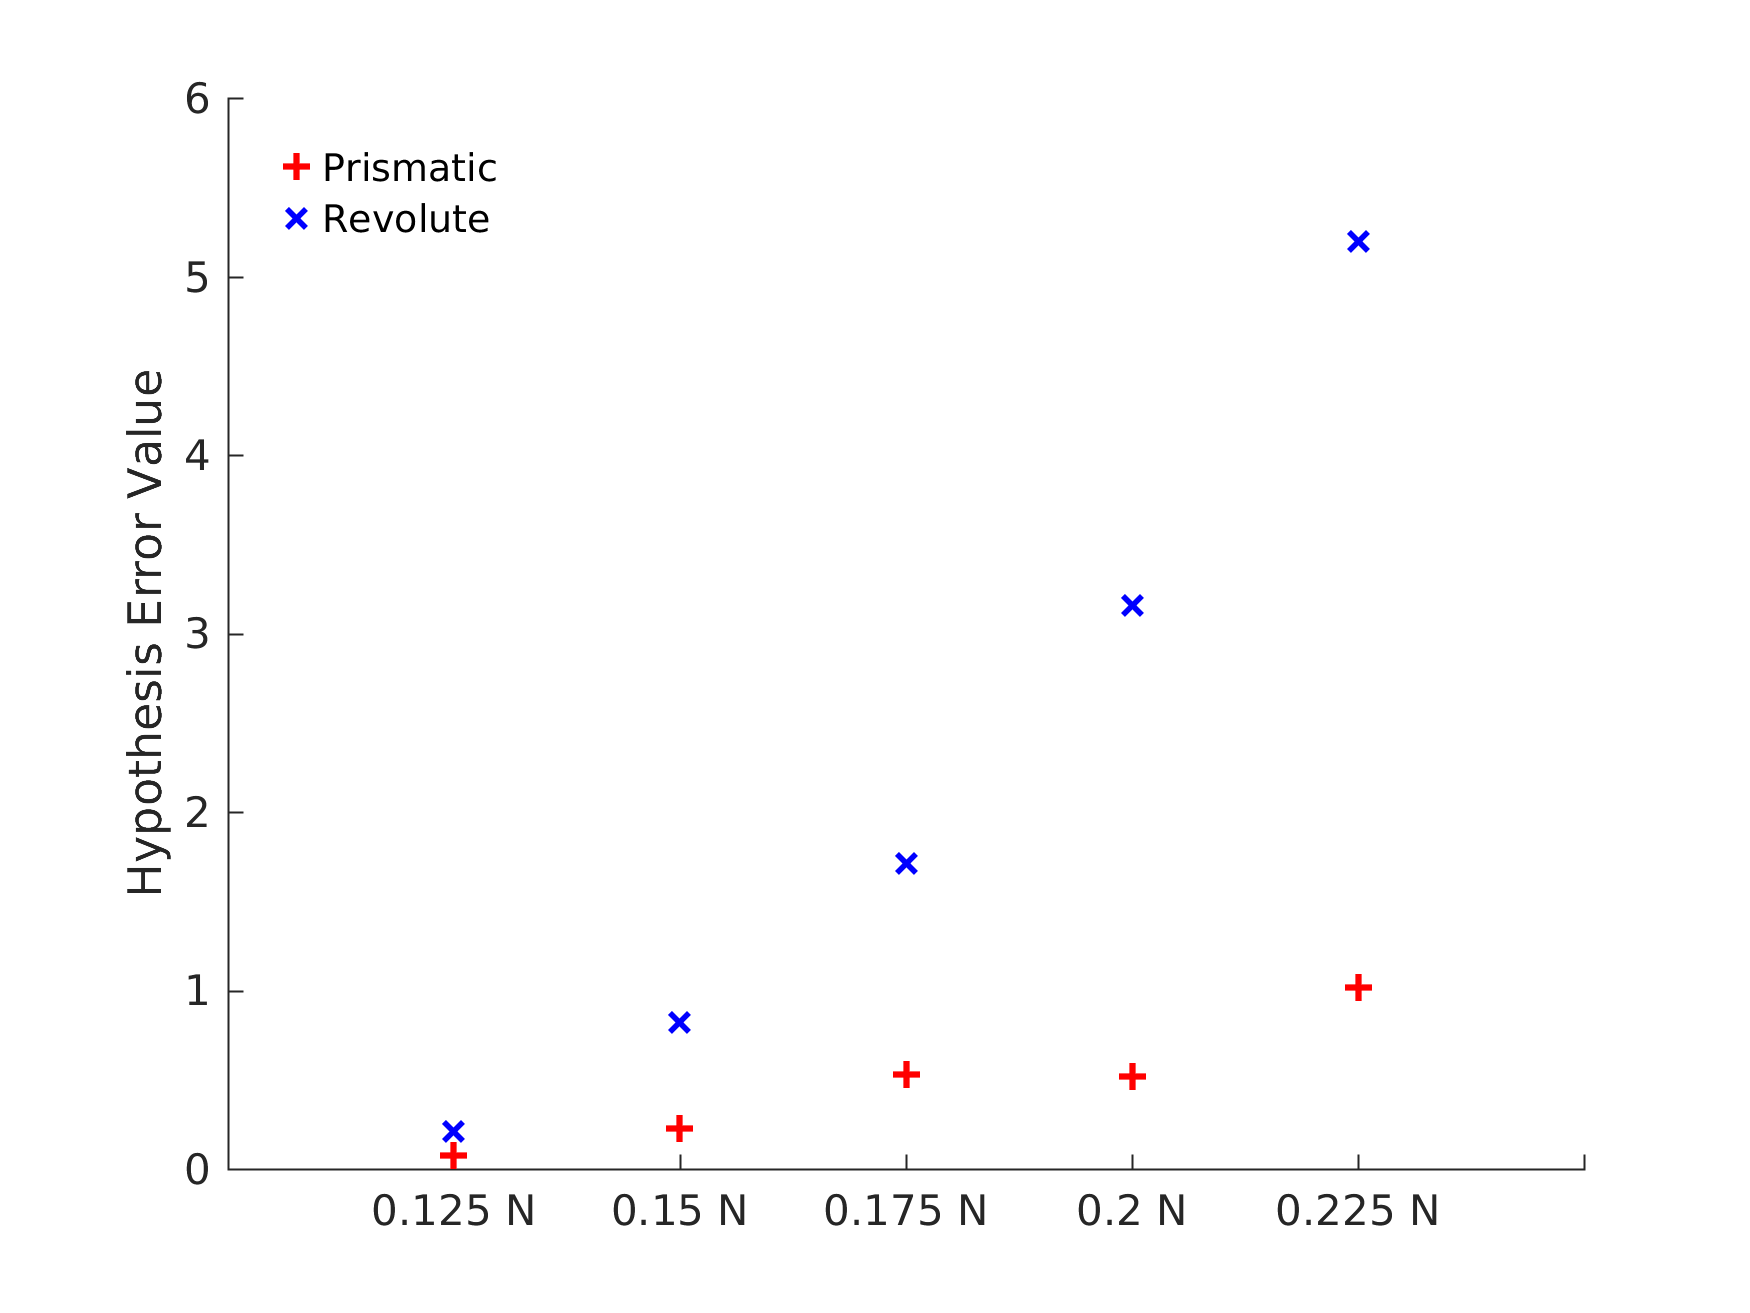
\includegraphics[width=0.55\textwidth]{figures/phypdiff.png}
  \caption{Prismatic Motion Hypothesis Error Value}
  \label{phypdiff}
\end{figure}

For the data of revolute joint motion under the influence of different forces, the Fig.(\ref{rhypdiff}) shows the value of $R_{hyp}$ is less than $P_{hyp}$. This indicates that for this joint motion, revolute articulation model is a close match to the actual joint type present in the articulated object.

\begin{figure}[H]
  \centering
  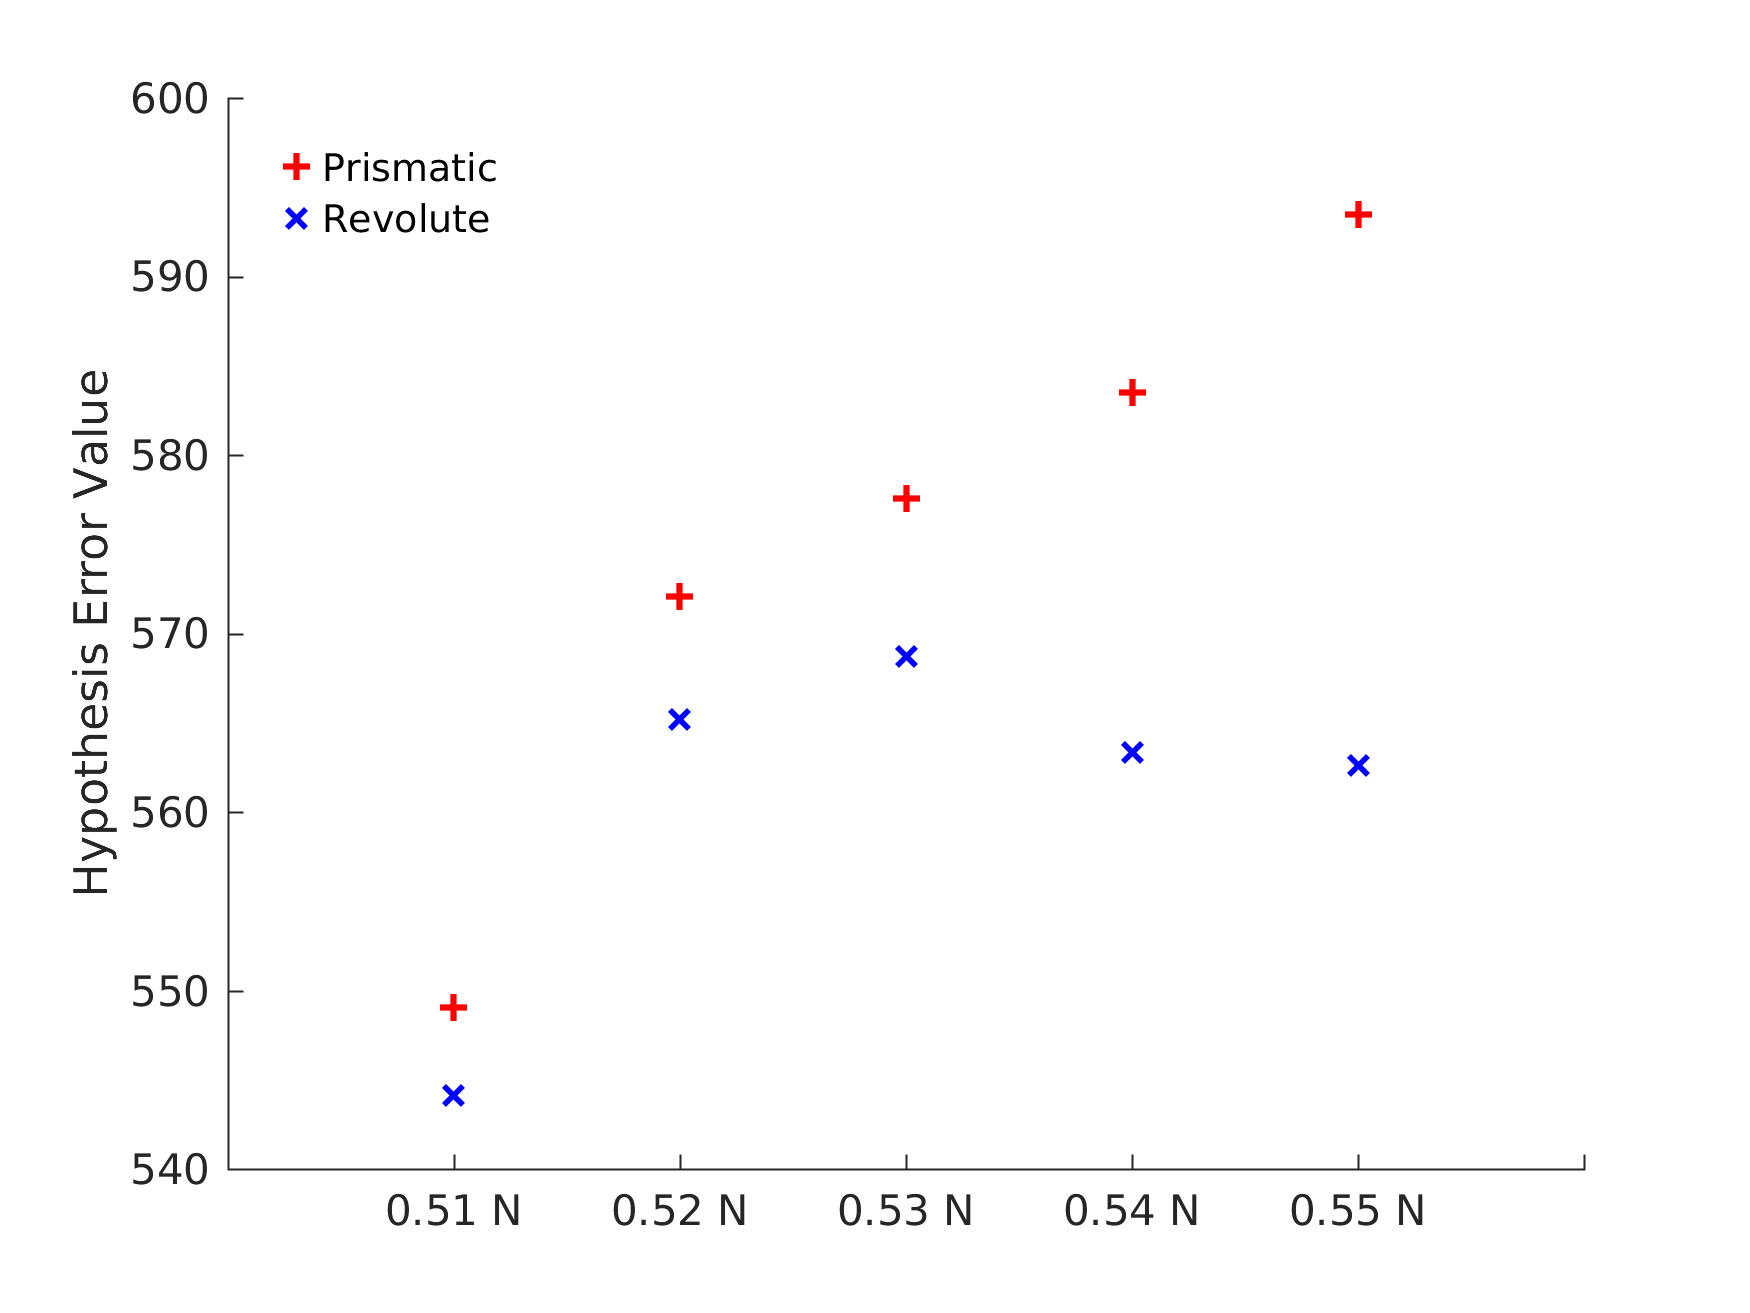
\includegraphics[width=0.55\textwidth]{figures/rhypdiff.png}
  \caption{Revolute Motion Hypothesis Error Value}
  \label{rhypdiff}
\end{figure}

Even though we made several assumptions about the availability of rigid body pose and inertial parameters of the object models, Gazebo is a fixed time-step simulator, of $1~ms$, which adds considerable numerical errors for a stiff mechanical  system considered in our experiments. In such a noisy environment, our work is a proof of concept proving that we can distinguish between articulation models using the kinematic evolution and interaction wrench information available while manipulating an articulated object.



\begin{landscape}
	\begin{figure}[!ht]
		\centering
		\caption{Gantt Chart PhD Year II}
		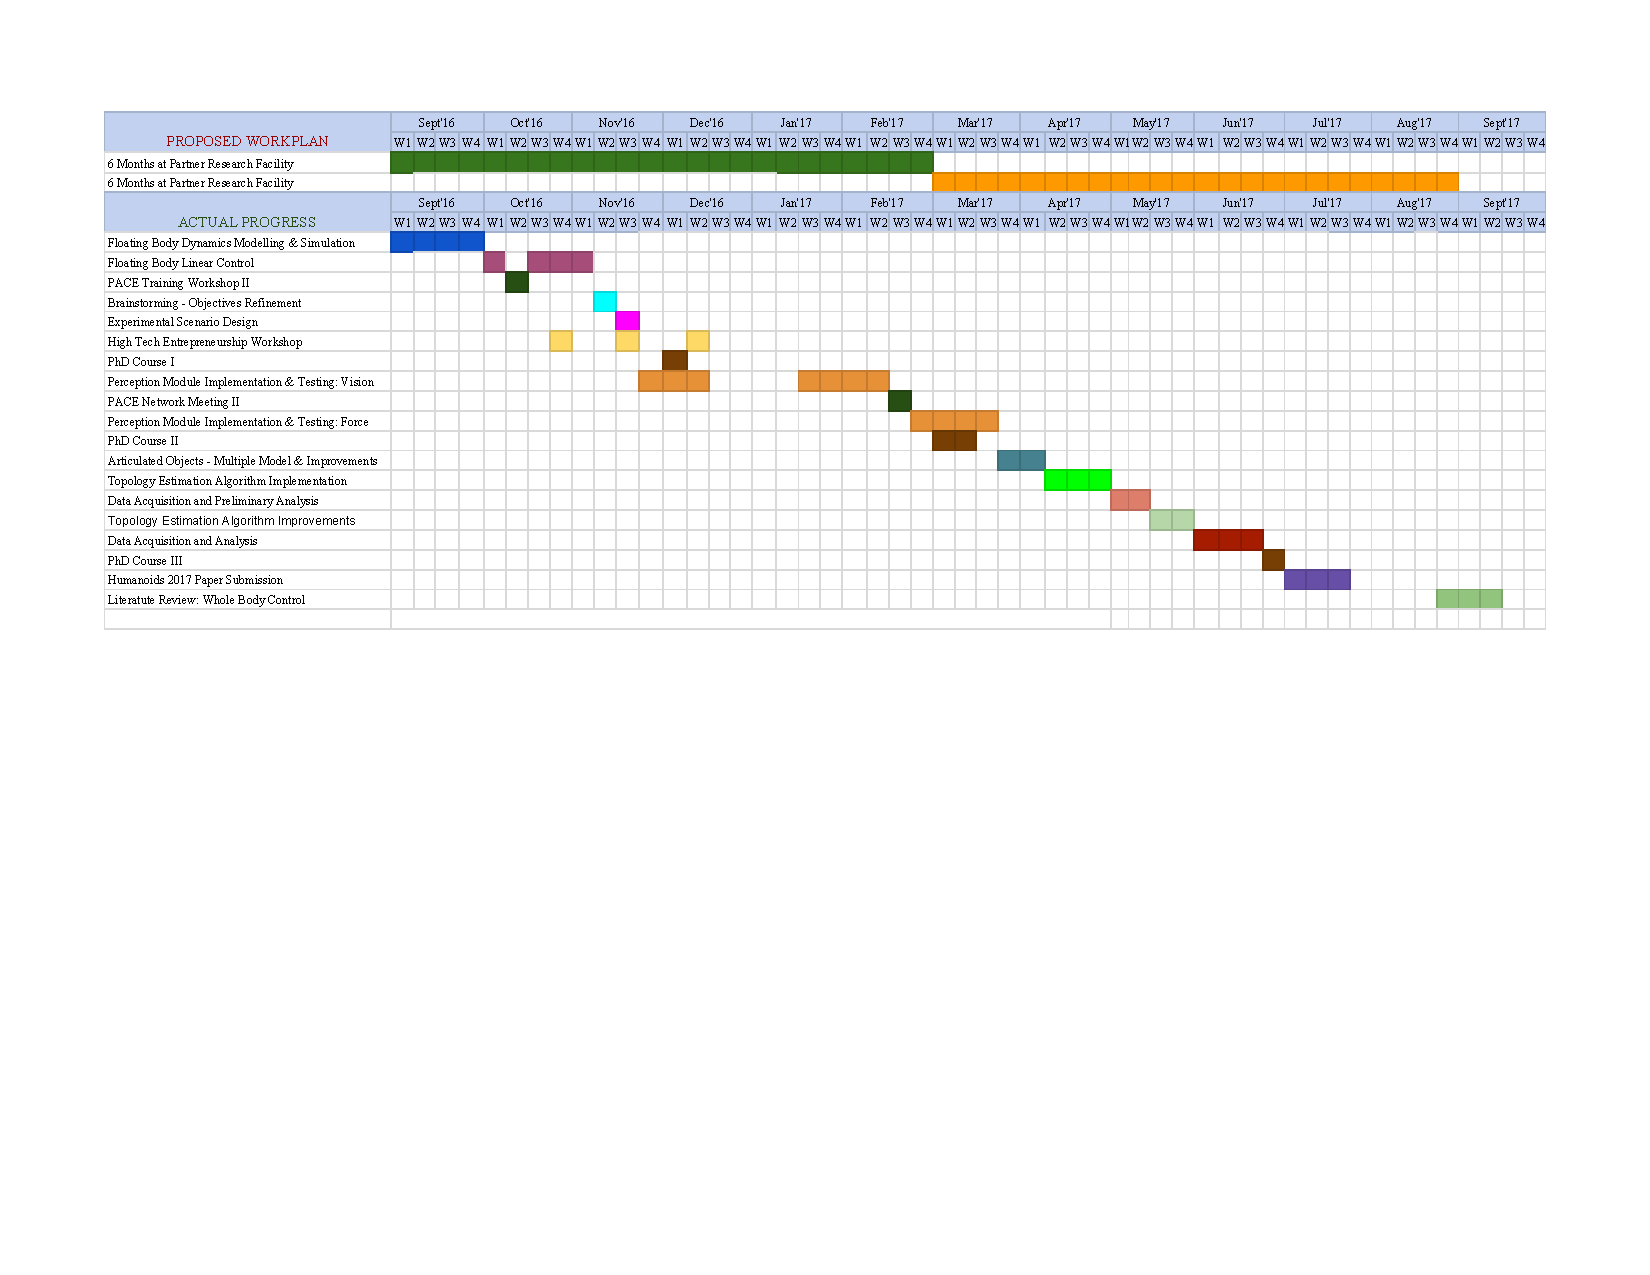
\includegraphics[scale=1]{PhD_year2_gantt.pdf}
		\label{gantt}
	\end{figure}
\end{landscape}

\renewcommand{\bibsection}{\subsection{\bibname}}
\renewcommand{\bibname}{\large{References}}
\bibliographystyle{plain}
\bibliography{ref}

\section{Traning Related to the PhD Programme}
\begin{enumerate}
    \item Artificial Cognitive Systems
    \begin{itemize}
		\item Type: PhD Course
		\item Organizer: IIT
		\item Duration: 10 Hours
		\item Credits: 3
		\item Verification: Pass
	\end{itemize}
	\item An Introduction to Spatial (6D) Vectors and Their Use in Robot Dynamics
	\begin{itemize}
		\item Type: PhD Course
		\item Organizer: IIT
		\item Duration: 15 Hours
		\item Credits: 5
		\item Verification: Pass
	\end{itemize}
	\item Machine Learning: A Computational Intelligence Approach
	\begin{itemize}
		\item Type: PhD Course
		\item Organizer: UNIGE
		\item Duration: 18 Hours
		\item Credits: 6
		\item Verification: EXAM TO BE HELD ON 18-SEP-2017
	\end{itemize}
\end{enumerate}
\section{Other Activities}
\begin{itemize}
    \item PACE second Thematic Workshop(TW2) on Active Inference at l’Université de Lyon, 12 - 14 October 2016, Lyon, France
    \item Online E-Learning module on Kinematic data (arm + eye): Concepts and analysis by Prof. Joan Lopez Moliner from Universitat de Barcelona (UB), 24 November 2016
    \item Workshop on High Tech Entrepreneurship organized by IIT and University of Genoa, 28 October - 15 December 2016, Genoa, Italy
    \item PACE Second Network Meeting(NM2) at  Universitat de Barcelona (UB), 20 - 22 February 2017, Barcelona, Spain
    \item Science communication project ~\cite{SCP} of PACE in partnership with the International School for Advanced Studies - SISSA, Trieste, Italy
    \item Online E-Learning module on Introduction to robotics and haptic device control by Prof. Gabriel Baud-Bovy from IIT, Italy, 4 May 2017
    \item Online E-Learning module on Haptic devices by Prof. Gabriel Baud-Bovy from IIT, Italy, 24 May 2017
    \item Online E-Learning module on Human-robot social interactions by Dr. Alessandra Sciutti from IIT, Italy, 15 June 2017
    \item Online E-Learning module on Robot assisted rehabilitation by Dr. Jacopo Zenzeri from IIT, Italy, 20 June 2017
    \item Online E-Learning module on Control theory dy Dr. Daniele Pucci from IIT, 29 June 2017
    \item Online E-Learning module on An example of and advanced robot: iCub by Prof. Giulio Sandini and Dr. Francesco Rea from IIT, Italy, 25 July 2017
\end{itemize}
\vspace*{10cm}
Signatures, \\
\vspace*{4cm}
PhD Student \hspace*{12cm} Tutor(s)

\end{document}
